\documentclass[a4paper,11pt,authoryear]{article}
\usepackage[utf8]{inputenc}
\usepackage{authblk}
\usepackage{cite}
\usepackage{csquotes}
\usepackage[T1]{fontenc}
\usepackage{graphicx}
\usepackage{hyperref}
\usepackage{listings}
\usepackage{lmodern}
\usepackage{ngerman}
\usepackage{xcolor}
\usepackage{xparse}

\NewDocumentCommand{\codeword}{v}{%
\texttt{\textcolor{blue}{#1}}%
}

\lstset{language=C,keywordstyle={\bfseries \color{blue}}}

\title{Installation von DDB Systemen}
\author[1]{Richard Neumann}
\affil[1]{HOMEINFO - Digitale Informationssysteme GmbH}

\begin{document}

\maketitle
\tableofcontents

\begin{abstract}
Dieses Dokument beschreibt das Zurückspielen von \emph{HOMEINFO Digital Signage Linux} (\emph{HIDSL}) Abbildern (\emph{Images}) auf TSPCs der Fa. MOStron zum Einsatz für das Produkt \emph{Das Digitale Brett} (\emph{DDB}).
\end{abstract}

\pagebreak

\section{Beziehen der ISO-Datei}
Einen Downloadlink zum jeweils aktuellen Image stellen wir Ihnen separat zu Verfügung.

\section{Erstellen des USB-Speichersticks}
Spielen Sie die heruntergeladene ISO-Datei auf einen USB-Speicherstick.
\textbf{ACHTUNG:} Beim Beschreiben des Zielmediums werden alle darauf befindlichen Daten unwiederbinglich gelöscht. Achten Sie daher unbedingt darauf, dass Sie das korrekte Zielmedium ausgewählt haben.
\subsection{Linux/Mac}
Auf unixoiden Systemen können Sie das Programm \codeword{dd} verwenden, um das Image auf den USB Stick zu schreiben.
\begin{verbatim}
  # dd if=/pfad/zur/iso/datei of=/pfad/zum/usb_stick; sync
\end{verbatim}
\subsection{Windows}
Unter Windows empfehlen wir die Benutzung des Programms \codeword{rufus}.
Es ist zu beachten, dass hier das Image im \emph{DD-Abbild-Modus} geschrieben werden muss \ref{fig:rufus} .
\begin{figure}
  \begin{center}
    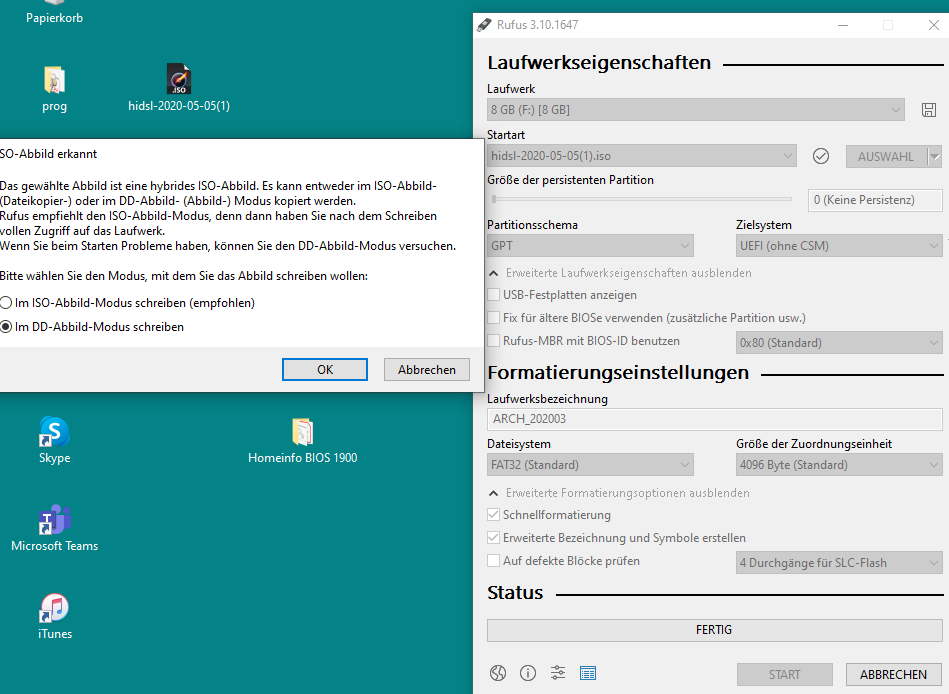
\includegraphics[scale=0.3]{ddb_rufus_win.png}
    \caption{Schreiben des Abbildes mittels Rufus unter Windows \cite{siebert_rufus}.}
    \label{fig:rufus}
  \end{center}
\end{figure}
\section{Booten des Systems vom USB-Stick}
Booten Sie das Gerät von dem erstellten USB-Stick. Herzu müssen Sie ggf. das korrekte Bootmedium am Gerät auswählen (F7 bei den neuen TSPC).

\section{Installation}
Um das gebootete System mit dem DDB-Image zu bespielen, führen Sie das Kommando \codeword{hirestore} aus.
Je nach System und dessen Zustand, können verschiedene Parameter notwendig sein.
\subsection{Installation auf UEFI Systemen}
Die Installation auf UEFI Systemen ist aktuell der Standard. Im Zweifel sollte diese Variante gewählt werden.
\begin{verbatim}
  # hirestore
\end{verbatim}
\subsection{Installation auf BIOS Systemen}
Die Installation auf BIOS Systemen für MBR-Boot sollte nur auf solchen Systemen durchgeführt werden, welche UEFI nicht unterstützen.
Dies sind beispielsweise die TSPCs aus der ersten DDB-Generation mit \emph{AMD G-T40E} Prozessoren.
\begin{verbatim}
  # hirestore -m
\end{verbatim}
\subsection{Fehlerbehebung}
Bei vorinstallierten Windows Systemen kann es manchmal dazu kommmen, dass \codeword{sgdisk} nicht erfolgreich ausgeführt werden konnte:
\begin{verbatim}
  [ERROR] hirestore: Command '['/usr/bin/sgdisk', '-og', '/dev/sda']' 
  returned non-zero exit status 2.
\end{verbatim}
In diesem Falle, führen Sie \codeword{hirestore} mit dem \emph{zusätzlichen} Parameter \codeword{-w} aus:
\begin{verbatim}
  # hirestore -w
\end{verbatim}
bzw.
\begin{verbatim}
  # hirestore -mw
\end{verbatim}
\subsection{Weitere Optionen}
Sie können sich alle unterstützten Parameter des Programms \codeword{hirestore} mittels des Parameters \codeword{-h} anzeigen lassen:
\begin{verbatim}
  # hirestore -h
\end{verbatim}

\section{Konfiguration}
Nach dem Zurückspielen des Images, starten Sie das System neu und wählen Sie im Bootloader den \emph{Configuration Mode}.
Führen Sie nach der automatischen Anmeldung als Benutzer \codeword{hidslcfg} in der Konsole folgendes Kommando aus:
\begin{verbatim}
  $ sudo hidslcfg (-S|-T|-P|-N)
\end{verbatim}
Wählen Sie dazu genau einen Hardware Typen aus:
\begin{itemize}
  \item \codeword{-S} MOStron TSPC Standard, 24 Zoll
  \item \codeword{-T} MOStron TSPC Standard, 32 Zoll
  \item \codeword{-P} MOStron TSPC Phönix, 24 Zoll
  \item \codeword{-N} MOStron TSPC Neptun, 24 Zoll
\end{itemize}
Sie können zudem über den Parameter \codeword{-u} direkt Ihren Benutzernamen angeben:
\begin{verbatim}
  $ sudo hidslcfg (-S|-T|-P|-N) -u <ihr_benutzername>
\end{verbatim}
\subsection{Wiedervergabe von System-IDs}
Standardmäßig erstellt \codeword{hidslcfg} beim Aufruf ein \emph{neues} System in der Datenbank.
Bei Reparaturfällen darf ausnahmsweise die System-ID an das reparierte Gerät wieder vergeben werden.
Um dies zu erlauben, müssen Sie den \emph{zusätzlichen} Parameter \codeword{-f} angeben:
\begin{verbatim}
  $ sudo hidslcfg (-S|-T|-P|-N) -f <system_id>
\end{verbatim}
bzw.
\begin{verbatim}
  $ sudo hidslcfg (-S|-T|-P|-N) -fu <ihr_benutzername> <system_id>
\end{verbatim}
Seien Sie bei der Wiedervergabe von System-IDs bitte vorsichtig!

\subsection{Fehlerbehebung}
Falls Sie die folgende Fehlermeldung erhalten:
\begin{verbatim}
  [CRITICAL] hidslcfg: You need to be root to run this script!
\end{verbatim}
so haben Sie womöglich vergessen, dem Kommando \codeword{hidslcfg} das Kommando \codeword{sudo} (s.o.) voranzustellen.
Letzteres erlaubt die Ausführung von \codeword{hidslcfg} als administrativer Benutzer, was für die korrekte Funktion vonnöten ist.
\subsection{Weitere Optionen}
Sie können sich alle unterstützten Parameter des Programms \codeword{hidslcfg} mittels des Parameters \codeword{-h} anzeigen lassen:
\begin{verbatim}
  $ hidslcfg -h
\end{verbatim}
Das Voranstellen von \codeword{sudo} ist in diesem Falle nicht notwendig.

\section{Abschluss der Installation}
Nach erfolgreicher Konfiguration können Sie das System herunterfahren oder neu starten.
Das System bootet standardmäßig in den \emph{Digital Signage Mode} und befindet sich dort im Auslieferungszustand im sog. \emph{Schwarzbildmodus}, welcher nur einen Cursor in Form eines Huhns anzeigt.
Mit diesem können Sie bei Bedarf die Touch-Funktion des Systems testen.

\section{Magic USB Key}
Mithilfe eines \emph{magischen} USB Sticks können Sie vordefinierte Konfigurationen auf das System übertragen lassen.
Der USB Speicherstick muss dabei mit \codeword{FAT32} formatiert sein und das Dateisystemlabel \codeword{DDBCFG} tragen.
Es werden die folgenden Konfigurationsdateien unterstützt, wobei auf Groß- und Kleinschreibung zu achten ist:

\subsection{WLAN}
Mittels der Datei \codeword{wifi.txt} können sie \emph{SSID} und \emph{PSK} für die WLAN Konfiguration vordefinieren.
Die Datei muss \codeword{UTF-8} codiert sein und über zwei Zeilen verfügen:
\begin{enumerate}
  \item \emph{SSID}
  \item \emph{PSK}
\end{enumerate}

Sie können diese Datei im Reiter \emph{WLAN} des grafischen Installers laden lassen.

\section{Migration von OpenVPN auf WireGuard}
Um ein vorhandenes System von \codeword{OpenVPN} auf \codeword{WireGuard} zu migrieren, führen Sie folgendes Kommando aus:
\begin{verbatim}
  $ sudo wgmigrate
\end{verbatim}
Auch hier können sie mittels des Parameters \codeword{-u} direkt Ihren Benutzernamen angeben:
\begin{verbatim}
  $ sudo wgmigrate -u <ihr_benutzername>
\end{verbatim}

\section{Reparatur des Dateisystems}
Falls ein System aufgrund von Dateisystemfehlern nicht mehr bootet, kann es mithilfe des Installationssticks repariert werden.
Dazu ist das System vom Installationsstick zu booten und anschließend das Kommando
\begin{verbatim}
  # fsck -y /dev/sda2
\end{verbatim}
bzw. auf Systemen mit MBR-Boot
\begin{verbatim}
  # fsck -y /dev/sda1
\end{verbatim}
auszuführen.
Abschließend kann das System neu gestartet werden.

\bibliography{references}{}
\bibliographystyle{plain}
\end{document}
